\documentclass{standalone}
\usepackage{tikz}
\usepackage{ctex,siunitx}
\setCJKmainfont{Noto Serif CJK SC}
\usepackage{tkz-euclide}
\usepackage{amsmath}
\usetikzlibrary{patterns, calc,3d}
\usetikzlibrary {decorations.pathmorphing,decorations.pathreplacing,decorations.shapes,}
\begin{document}
\small
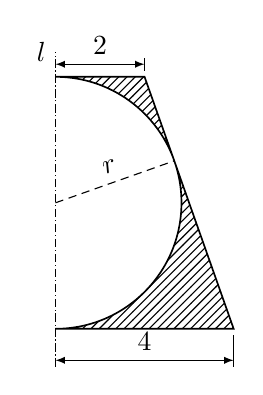
\begin{tikzpicture}[>=latex,scale=0.8]
  \draw[semithick,pattern=north east lines](0,2)--({sqrt(2)},2)--({2*sqrt(2)},-2)--(0,-2)arc(-90:90:2);
  \draw[densely dashdotted](0,-2.6)--(0,2.4)node[left]{$l$};
  \draw[very thin,<->](0,2.2)--({sqrt(2)},2.2)node[midway,above]{2};
  \draw[very thin,<->](0,-2.5)--({2*sqrt(2)},-2.5)node[midway,above]{4};
  \draw[very thin]({2*sqrt(2)},-2.1)--({2*sqrt(2)},-2.6)({sqrt(2)},2.1)--({sqrt(2)},2.3);
  \draw[densely dashed](0,0)--(19.4712:2)node[midway,above,sloped]{$r$};
\end{tikzpicture}
\end{document}